\documentclass[12pt]{article}

 \usepackage{graphics}


\usepackage{geometry}
  \geometry{
    a4paper,
    total={6in, 9in},
    top=20mm,
  }

\usepackage{graphicx}
\graphicspath{ {./img/} }

\usepackage{array}
\newcolumntype{P}[1]{>{\centering\arraybackslash}p{#1}}

\usepackage{multirow}
\usepackage{subcaption}
\usepackage{hyperref}

\usepackage{pgfplots}
\pgfplotsset{width=5in,compat=1.9}

\title{Tema 1' Algoritmi genetici}
\author{Renghiuc Bianca Elena si Culbece Rose-Marie 2A2}
\date{01.11.2022}

\begin{document}

\maketitle
\section*{Abstract}

În raportul următor, vom determina punctul maxim al funcției $f(x)=x^3-60x^2-900x+100$ în intervalul [0, 31] prin metodele \textbf{Hill Climbing - First Improvement} și \textbf{Hill Climbing - Best Improvement}.

\section{Introducere}


Problema presupune găsirea maximului global al unei funcții, iar scopul este observarea bazinelor de atracție a maximelor locale. În graficul de mai jos, am reprezentat funcția ce urmează a fi studiată: \\



\begin{tikzpicture}
\begin{axis}[
    xmin = 0, xmax = 32,
    ymin = 0, ymax = 4200]
    \addplot[
        domain = 0:32,
    ] {x*x*x-60*x*x+900*x+100};
\end{axis}
\end{tikzpicture}


\section{Metode}

Hill Climbing este un algoritm eficient, euristic folosit pentru probleme de optimizare matematice. Acesta este util în găsirea optimelor globale. \\*
Am folosit două metode: {\textbf{Hill Climbing - First Improvement}} și {\textbf{Hill Climbing - Best Improvement}},   \\*

Pentru a reprezenta numerele am folosit un vector de 5 biți ce reprezintă punctul în care calculăm valoarea funcției. Pentru a afla vecinii am negat pe rând fiecare bit din vector. Am folosit un număr de 10000 de iterații. Iar algoritmul a fost repetat de 30 de ori.
Pentru varianta First Improvement am luat primul vecin generat prin negarea de biți, iar pentru cea Best Improvement am luat cel mai bun dintre vecini (cel mai mare).


\section{Rezultate}
Mai jos am realizat un tabel ce conține fiecare bazin de atracție și mulțimea de puncte inițiale pentru care căutarea ne duce spre același optim. 


\begin{center}
  \begin{tabular}{ |P{4cm}|P{12cm}| }
      
    \hline
    \multicolumn{2}{|c|}{ \textbf{First Improvement} } \\
    
    \hline
      Bazin de atracție & Punctele sale \\
    \hline

    3236     & 0, 1, 2, 3, 16, 17, 18, 19\\   
                \hline
    3803    &  7, 15, 23, 31\\
                \hline
    3988   &  4, 8, 12, 20, 24, 28\\
                \hline
    4100 & 5, 6, 9, 10, 11, 13, 14, 21, 22, 25, 26, 27, 29, 30\\

    \hline
  \end{tabular}
\end{center}

\begin{center}
  \begin{tabular}{ |P{4cm}|P{12cm}|}
      
    \hline
    \multicolumn{2}{|c|}{ \textbf{Best Improvement} } \\
    
    \hline
       Bazin de atracție & Punctele sale\\
    \hline

    3236   &  16, 17, 18, 19, 20\\
                
                \hline
    3803   &  6, 7, 22, 23\\
                \hline
    3988   &  4, 12, 28\\
                \hline
    4100   &  0, 1, 2, 3, 5, 8, 9, 10, 11, 13, 14, 15, 21, 24, 25, 26, 27, 29, 30, 31\\

    \hline
  \end{tabular}
\end{center}


\section{Comparatii}
Mai departe vom vedea care sunt diferențele dintre algoritmi. HC - Best Improvement alege mereu vecinul cel mai bun, iar HC - First Improvement îl alege pe primul. 

În acest grafic se poate observa câte valori are fiecare mulțime a bazinelor de atracție pentru fiecare din cele două metode prezentate.


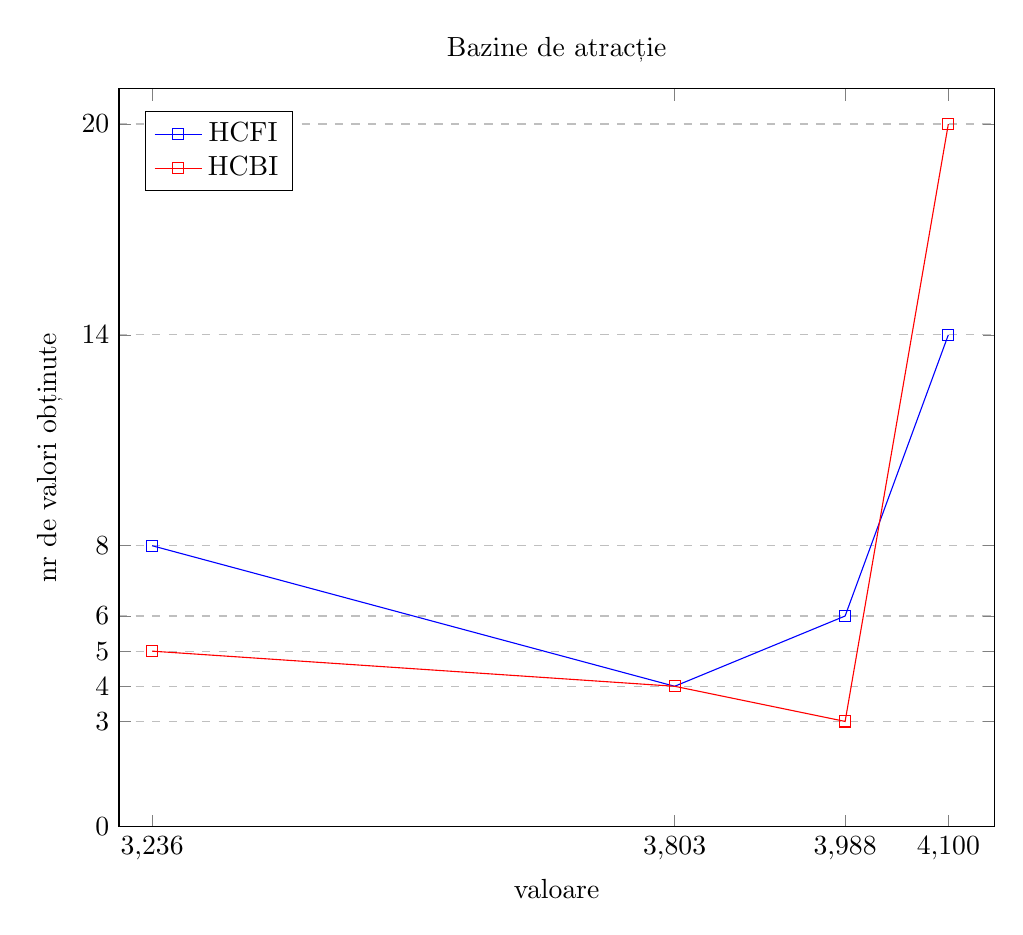
\begin{tikzpicture}
  \begin{axis}[
      title={Bazine de atracție},
      xlabel={valoare},
      ylabel={nr de valori obținute},
      xmin=3200, xmax=4150,
      ymin=0, ymax=21,
      xtick={3236, 3803, 3988, 4100},
      ytick={0, 3, 4, 5, 6, 8, 14, 20},
      legend pos=north west,
      ymajorgrids=true,
      grid style=dashed,
  ]
  
  \addplot[
      color=blue,
      mark=square,
      ]
      coordinates {
      (3236, 8)(3803, 4)(3988, 6)(4100, 14)
      };
      \addlegendentry{HCFI}
      
  \addplot[
      color=red,
      mark=square,
      ]
      coordinates {
      (3236, 5)(3803, 4)(3988, 3)(4100, 20)
      };
      \addlegendentry{HCBI}

      
  \end{axis}
\end{tikzpicture}

Utilizând algoritmul HC - First Improvement am găsit maximul global de 14 ori, iar utilizând algoritmul HC - Best Improvement am găsit maximul global de 20 ori din 32 de valori încercate.

\section{Concluzie}

În concluzie, testând cei doi algoritmi euristici enumerați la început putem ajunge la concluzia că versiunea Best Improvement este mai bună decat cea First Improvement. 

\begin{thebibliography}{9}
  \bibitem{}
    \url{https://profs.info.uaic.ro/~eugennc/teaching/ga/}
  \bibitem{}
    \url{https://en.wikipedia.org/wiki/Hill_climbing}
  \bibitem{}
    \url{https://latexdraw.com/plot-a-function-and-data-in-latex/}
  
  \end{thebibliography}  
  


\end{document}
